% Created 2025-04-28 Mon 23:18
% Intended LaTeX compiler: xelatex
\documentclass[a4paper,10pt,onecolumn,oneside,openright]{article}
\usepackage[no-math]{fontspec}
\usepackage[utf8x]{inputenc}
\newfontfamily\cyrillicfont{CMU Serif}
\newfontfamily\cyrillicfontsf[Script=Cyrillic]{Linux Libertine O}
\newfontfamily\cyrillicfonttt[Script=Cyrillic]{Hack}
\setmainfont[
  Ligatures=TeX,
  Extension=.otf,
  BoldFont=cmunbx,
  ItalicFont=cmunti,
  BoldItalicFont=cmunbi,
]{cmunrm}
\usepackage[Latin,Cyrillics]{ucharclasses}
\setTransitionsForCyrillics{\begingroup\cyrillicfont}{\endgroup}
\usepackage{polyglossia}
\setdefaultlanguage[variant=british]{english}
\setotherlanguage{latin}
\setotherlanguage{greek}
\setotherlanguage{russian}
\setotherlanguage{polish}
\setotherlanguage{german}
\setotherlanguage{ukrainian}
\newcommand{\RU}[1]{\foreignlanguage{russian}{#1}}
\usepackage{url}
\usepackage{listings}
\usepackage{array}
\usepackage{tabularx}
\newenvironment{conditions}
  {\par\vspace{\abovedisplayskip}\noindent
   \begin{tabular}{>{$}l<{$} @{} >{${}}c<{{}$} @{} l}}
  {\end{tabular}\par\vspace{\belowdisplayskip}}
\newenvironment{conditions*}
  {\par\vspace{\abovedisplayskip}\noindent
   \tabularx{\columnwidth}{>{$}l<{$} @{}>{${}}c<{{}$}@{} >{\raggedright\arraybackslash}X}}
  {\endtabularx\par\vspace{\belowdisplayskip}}
\usepackage[tableposition=t]{caption}
\captionsetup[table]{skip=8pt}
\usepackage{pdflscape}
\usepackage[tableposition=t]{caption}
\usepackage{amsmath}
\usepackage{amssymb}
\usepackage{amsbsy}
\usepackage{amsfonts}
\usepackage{soul}
\usepackage{xunicode}
\usepackage[normalem]{ulem}
\usepackage{fixltx2e}
\usepackage[unicode]{hyperref}
\usepackage{cleveref}
\newcommand*{\fullref}[1]{\hyperref[{#1}]{\ref*{#1} \nameref*{#1}}}
\newcommand*{\fullRef}[1]{\nameCref{#1} \hyperref[{#1}]{\ref*{#1} \nameref*{#1}}}
\newcommand*{\fullREF}[1]{\nameCref{#1} \ref{#1}: \nameref*{#1}}
\newcommand*{\FullREF}[1]{\nameCref{#1} \ref{#1} (\nameref*{#1})}
\newcommand*{\eqnCref}[1]{\nameCref{#1} \ref{#1}}
\newcommand*{\EqnCref}[1]{\nameCref{#1} \ref*{#1}}
\usepackage{newunicodechar}
\newunicodechar{^^^^2139}{\textbf{i}}
\newcommand{\citinf}{{\newline\hspace*{\fill}}\textasteriskcentered}
\newcommand{\citfix}{{\hspace*{\fill}}\textasteriskcentered}
\newcommand{\citsrc}{{\vadjust{\vspace{8pt}}\nolinebreak\hspace{\fill}\mbox{}\linebreak\hspace*{\fill}\textemdash\space}}
\usepackage{mathtools}
\usepackage{amsthm}
\usepackage{nicefrac}
\usepackage{amscd}
\usepackage{amstext}
\usepackage{threeparttable}
\AtBeginDocument{\hypersetup{pdfauthor={Jan Nikadon},pdftitle={\thetitle},pdfsubject={subject},pdfkeywords={keyword1,}{keyword2},}}
\hypersetup{xetex,colorlinks=true,linktocpage=true,linkcolor=RoyalPurple,citecolor=RoyalPurple,filecolor=RoyalBlue,urlcolor=RoyalBlue,pagebackref=true,plainpages=false,pdfpagelabels=true,bookmarksnumbered=true,}
\PassOptionsToPackage{dateabbrev=false,natbib=true,style=apa,backref=true,backrefstyle=two,dashed=false,hyperref=true,backend=biber,maxbibnames=99,firstinits=true,giveninits=false,uniquename=init,citetracker=true,parentracker=true,url=false,doi=true,}{biblatex}
\usepackage{biblatex}
\usepackage[newfloat]{minted}
\usepackage{graphicx}
\usepackage{longtable}
\usepackage{float}
\restylefloat{table}
\usepackage{titling}
\usepackage[usenames,dvipsnames,svgnames]{xcolor}
\definecolor{fuchsiapink}{rgb}{1.0, 0.47, 1.0}
\definecolor{cream}{rgb}{1.00, 0.99, 0.82}
\definecolor{champagne}{rgb}{0.97, 0.91, 0.81}
\definecolor{beaublue}{rgb}{0.74, 0.83, 0.9}
\definecolor{blanchedalmond}{rgb}{1.0, 0.92, 0.8}
\definecolor{brilliantlavender}{rgb}{0.96, 0.73, 1.0}
\addbibresource{~/cc/org/roam/refs/core/core-Base.bib}
\addbibresource{base.bib}
\date{}
\title{README}
\begin{document}

\maketitle
\section{Notes}
\label{sec:org0a92b78}
\begin{itemize}
\item PDF and BIB files: \url{./aux-refs/}
\item Parcellations/annotations \url{./aux-annots/fsaverage/label/}
\item All parcellations transformed to \texttt{fsaverage}:
\begin{itemize}
\item \texttt{?h.aparc.annot}
\begin{itemize}
\item Desikan-Killiany Atlas \parencite{r2006PaperDesikanEtAlN2}
\item Available as a standard option in FreeSurfer/MNE distribution
\end{itemize}
\item \texttt{?h.aparc\_sub.annot}
\begin{itemize}
\item A more detailed version of the Desikan-Killiany Atlas
\parencite{r2006PaperDesikanEtAlN2}
\item Includes sub-parcellations based on
\textcite{r2018PaperKhanEtAlN2}
\begin{itemize}
\item QUOTE: \textbf{Cortical parcellation (labels)} \emph{FreeSurfer was
used to automatically divide the cortex into 72 regions}
\parencite{r1999PaperDaleEtAlN2}. \emph{After discarding “medial
wall” and “corpus callosum”, these regions were further
divided in to a total of N = 448 cortical “labels (Fig.
S4)”, so that each label covers a similar area again using
FreeSurfer. \uline{We employed this high-resolution parcellation
scheme because cortical surface is very convoluted and
averaging across a large label, which crosses multiple
sulci and gyri, can result in signal cancellation across
the parcel}. Lastly, \uline{a high-resolution parcellation also
reduces the dependence of the results on the specific
selection of the parcels}.}
\end{itemize}
\item NB: Recently used in \textcite{r2025PaperRuuskanenAvendano-DiazN1}
\begin{itemize}
\item Sub-parcellations were methodologically justified in the
context of addressing the same problem we face
\item QUOTE: \textbf{Cortical parcellation} \emph{To decrease computational
complexity and increase interpretability, we employed a
cortical parcellation to reduce the dimensionality of the
source-space data. To that end, the data were organized
into 448 ROIs as defined in the aparc sub parcellation
scheme developed by Khan and colleagues
\parencite{r2018PaperKhanEtAlN2} based on the
Desikan–Killiany atlas}.
\item QUOTE: \emph{The time courses within each ROI were then
averaged to form a representative time series. To prevent
signal cancellation at the opposite sides of sulci, a
sign-flip operation was applied to the signals of the
sources whose orientation differed from the dominant
direction within the ROI by more than 90◦. The use of a
relatively dense parcellation further reduces signal
cancellation and flattening during the averaging
procedure}.
\item \begin{center}
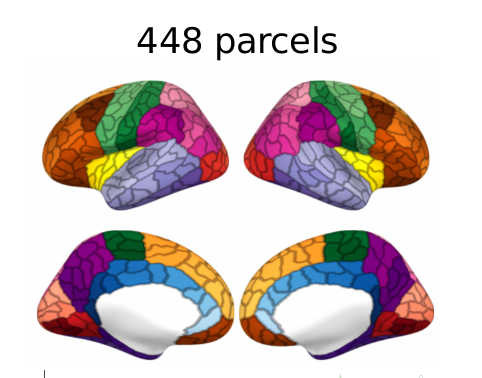
\includegraphics[width=.9\linewidth]{aux-imgs/r2025PaperRuuskanenAvendano-DiazN1-img-0001.png}
\end{center}
\item BTW: ↓ Not a bad template for localization visualization (if
one adds a histogram to such circle).
\item \begin{center}
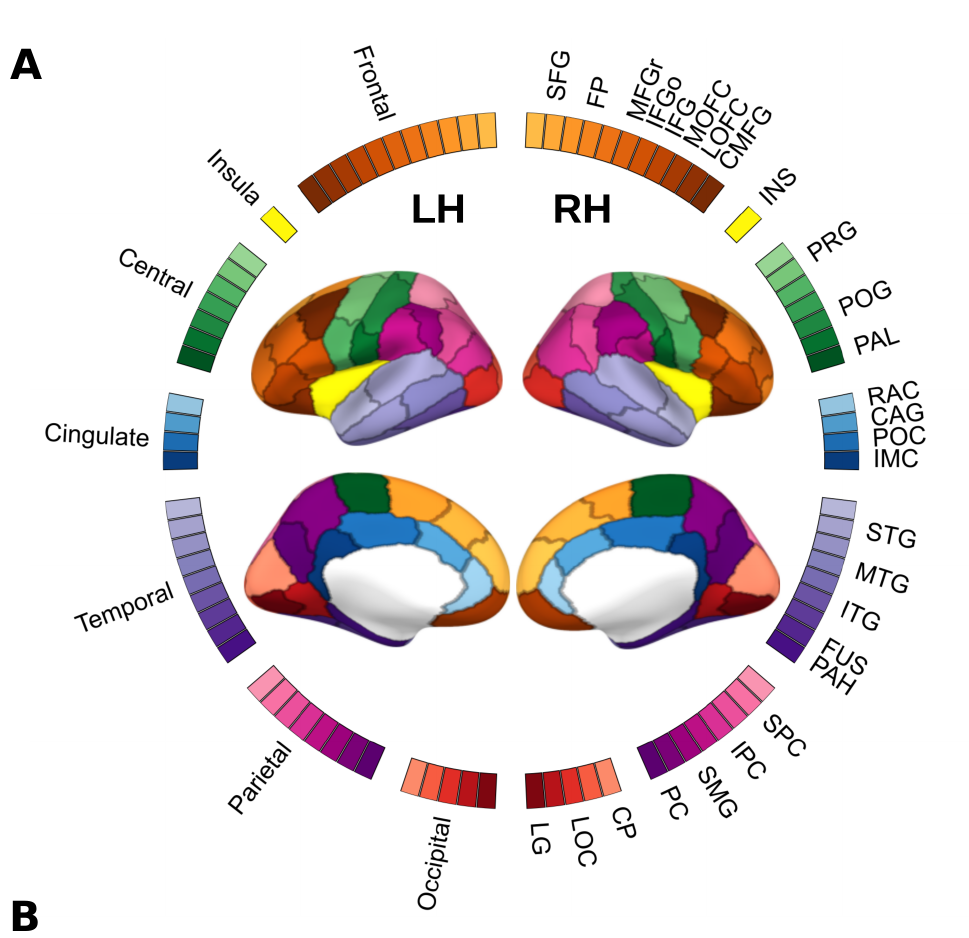
\includegraphics[width=.9\linewidth]{aux-imgs/r2025PaperRuuskanenAvendano-DiazN1-img-0002.png}
\end{center}
\end{itemize}
\item NB: Interesingly, both \textcite{r2018PaperKhanEtAlN2} and
\textcite{r2025PaperRuuskanenAvendano-DiazN1} relied on \texttt{?h.aparc\_sub.annot}
to solve a problems very similar to the ones we
discossed today.
\item \texttt{BTW: ?h.aparc\_sub\_FIXED.annot} contains manually corrected label strings.
\end{itemize}
\item \texttt{?h.HCPMMP1.annot}
\begin{itemize}
\item From \textcite{r2016PaperGlasserEtAlN1}
\item A strong alternative candidate for consideration.
\item \texttt{?h.HCPMMP1\_ORIG.annot} is OK
\end{itemize}
\item \texttt{?h.power.annot}
\begin{itemize}
\item From \textcite{r2011PaperPowerEtAlN2}
\item Not a preferred option for my taste (although, just in case,
please find it in the fsaverage space)
\item This parcellation is highly non-uniform in parcel size; some
areas are very small, while others cover large cortical
surface regions (likely due to idiosyncratic data used, which
may reflect their specific dataset but is suboptimal for
exploring new data).
\end{itemize}
\end{itemize}
\end{itemize}
\section*{References}
\label{sec:org16a3bab}
\addcontentsline{toc}{section}{References}

\printbibliography[heading=none]
\end{document}
